\documentclass[convert={ghostscript,gsdevice=tiffg4,
outext=.tiff,density=1200}]{standalone}
    \usepackage{tikz}
    \usepackage{pgfplots}
    \usetikzlibrary{patterns}
\mathversion{bold}
\begin{document}
\large
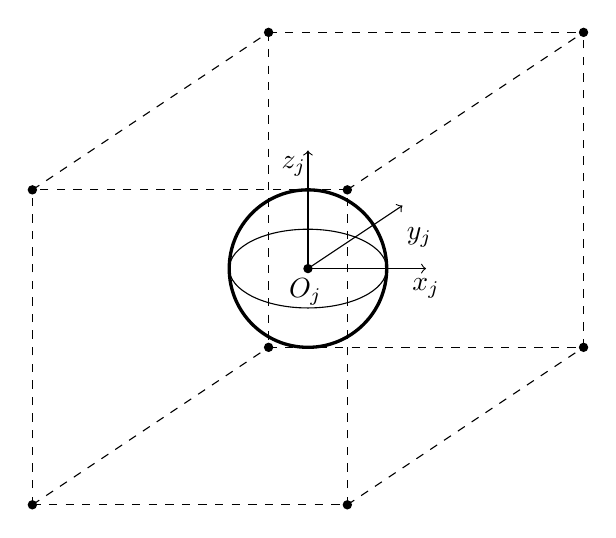
\begin{tikzpicture}%[scale=1.5]
\draw[->] (3.5,3) -- (4.7,3.8) node[anchor=north] {};
\draw[->] (3.5,3) -- (3.5,4.5) node[anchor=east] {};
\draw[->] (3.5,3) -- (5,3) node[anchor=north] {$x_j$};

\node[left] at (3.8,2.7) {$O_j$};
\node[left] at (5.2,3.4) {$y_j$};
\node[left] at (3.6,4.3) {$z_j$};
%\node[above right] at (0.85,0) {$A$};
%\node[above left] at (3.15,0) {$B$};

\draw[very thick] (3.5,3) circle (1.0);
\draw (3.5,3) ellipse (1.0 and .5);

%\draw[very thick] (3,2) circle (1.0);
%\draw (3,2) ellipse (1.0 and .5);
%
%\draw[very thick] (0,3) circle (1.0);
%\draw (0,3) ellipse (1.0 and .5);
%
%\draw[very thick] (3,5) circle (1.0);
%\draw (3,5) ellipse (1.0 and .5);
%
%
%\draw[very thick] (4,0) circle (1.0);
%\draw (4,0) ellipse (1.0 and .5);
%
%\draw[very thick] (7,2) circle (1.0);
%\draw (7,2) ellipse (1.0 and .5);
%
%\draw[very thick] (4,3) circle (1.0);
%\draw (4,3) ellipse (1.0 and .5);
%
%\draw[very thick] (7,5) circle (1.0);
%\draw (7,5) ellipse (1.0 and .5);
%
%\draw[very thick] (8,0) circle (1.0);
%\draw (8,0) ellipse (1.0 and .5);
%
%\draw[very thick] (11,2) circle (1.0);
%\draw (11,2) ellipse (1.0 and .5);
%
%\draw[very thick] (8,3) circle (1.0);
%\draw (8,3) ellipse (1.0 and .5);
%
%\draw[very thick] (11,5) circle (1.0);
%\draw (11,5) ellipse (1.0 and .5);

\draw[dashed] (0,0) -- (3,2);
\draw[dashed] (0,0) -- (0,4);
\draw[dashed] (3,6) -- (3,2);
\draw[dashed] (0,0) -- (4,0);
\draw[dashed] (0,4) -- (3,6);
\draw[dashed] (4,0) -- (4,4);
\draw[dashed] (4,4) -- (0,4);
\draw[dashed] (4,4) -- (7,6);
\draw[dashed] (4,0) -- (7,2);
\draw[dashed] (7,2) -- (7,6);
\draw[dashed] (3,2) -- (7,2);
\draw[dashed] (3,6) -- (7,6);
%\draw[dashed] (4,0) -- (8,0);
%\draw[dashed] (4,4) -- (8,4);
%\draw[dashed] (7,6) -- (11,6);
%\draw[dashed] (7,2) -- (11,2);
%\draw[dashed] (8,0) -- (8,4);
%\draw[dashed] (11,2) -- (11,6);
%\draw[dashed] (8,0) -- (11,2);
%\draw[dashed] (8,4) -- (11,6);


\node[circle, fill=black, inner sep=1.2pt] at (0,0) {};
\node[circle, fill=black, inner sep=1.2pt] at (3,2) {};
\node[circle, fill=black, inner sep=1.2pt] at (0,4) {};
\node[circle, fill=black, inner sep=1.2pt] at (3,6) {};

\node[circle, fill=black, inner sep=1.2pt] at (4,0) {};
\node[circle, fill=black, inner sep=1.2pt] at (7,2) {};
\node[circle, fill=black, inner sep=1.2pt] at (4,4) {};
\node[circle, fill=black, inner sep=1.2pt] at (7,6) {};

%\node[circle, fill=black, inner sep=1.2pt] at (8,0) {};
%\node[circle, fill=black, inner sep=1.2pt] at (11,2) {};
%\node[circle, fill=black, inner sep=1.2pt] at (8,4) {};
%\node[circle, fill=black, inner sep=1.2pt] at (11,6) {};

\node[circle, fill=black, inner sep=1.2pt] at (3.5,3) {};


%\node[circle, fill=black, inner sep=1.2pt] at (1,0) {};
%\node[circle, fill=black, inner sep=1.2pt] at (3,0) {};

\end{tikzpicture}
\end{document}

%%% Local Variables: 
%%% mode: latex
%%% TeX-master: t
%%% End: 
